\chapter{Sustainable Development}
\label{ch:sustaindev}
\setlength{\parindent}{15pt}

Cradle to Cradle tool has been discarded due to the fact that certain materials such as carbon fibre composites and electronic components cannot be recycled to a raw material phase completely. Thus, only Life Cycle Assessment (LCA) is considered from this point of the project. The technical framework for LCA can be seen in \autoref{fig:lcatriangle}. It starts with the central block, 'Goal and Scope', then can flow into Impact Assessment and Inventory Analysis \cite{lca}.

\begin{figure}[H]
    \centering
    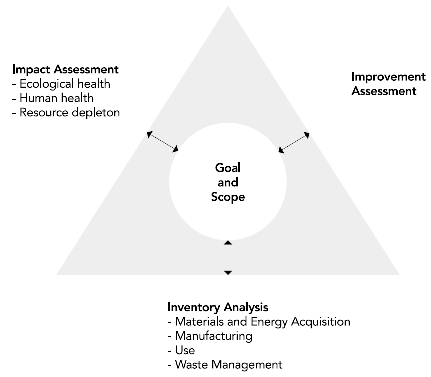
\includegraphics[width=0.6\textwidth]{SustainableDev/Figures/LCAtriangle.pdf}
    \caption{Technical Framework for Life Cycle Assessment}
    \label{fig:lcatriangle}
\end{figure}


\section{Goal and Scope}
The goal and scope definitions need to be determined as a first process of a LCA. The following paragraphs elaborate on details of each aspect of the first process. 

\paragraph{Goal} A mission need statement (MNS) can be used to define the goal. The MNS states, 'Carry out both supervised and autonomous monitoring and transport missions, comprising vertical take-off and landing, and high-velocity in horizontal flight.'

\paragraph{Scope} Since the project will stretch to planning of production of the UAV, it is important to define detailed assessment methods to be used. In order to define the assessment methods, a system to be studied and system boundaries need to be determined. Functions of the system have been identified based on a functional breakdown structure in the baseline report\cite{baseline}. 

\begin{itemize}
    \item Perform air transport
    \item Perform various missions
    \item Perform missions under various conditions
\end{itemize}

\paragraph{Functional Unit}
A main purpose for a functional unit is to set a normalised basis of comparison. For a consistent analysis, it is decided that further quantitative comparison will have a normalised scale from 0 to 100.

\paragraph{System Boundaries}
System boundaries are defined based on requirements, which can be found in \autoref{ch:requ}.

\paragraph{Data Quality}
Data quality in LCA is reflected in the final LCA. At this point of the stage, it is not possible to come up with a consistent and traceable data quality, such as time-related coverage, geographical coverage and technological coverage\cite{lca}. It will be established in the next phase of the project. 

\paragraph{Critical Review Process}
Critical review process is not applicable to this project, since the process is mainly for certification of a system or product and publication of the project in terms of environmental standards.

\section{Inventory Analysis}
Inventory analysis is carried out after defining goal and scope definition. A robust and qualitative inventory analysis can be carried out, as sustainability analysis is done and a production plan for the final concept is constructed.

\subsection{Materials and Energy Acquisition}
Relevant quantitative data has to be collected, but it is not possible at this point of the project, as parts of the UAV are not specified down to depth of types of materials and dimensions. Inputs and outputs of a product system need to be identified in order to identify materials and energy acquisition. In order to construct a UAV, raw materials are taken and processed into parts. Inputs during this stage are raw materials, energy spent to process raw materials into parts, labour and machines used for processing and production, while outputs can be parts or products. According to \autoref{ch:sustain}, chosen materials are EPP (polypropylene), aluminium and carbon fibre (polymer variants). Transforming raw materials into parts can be done by using thermal and kinetic energy, based on a type of manufacturing and process methods. The thermal and kinetic energy can be obtained by operating relevant machines using fossil fuel and stored electricity from a power plant.

\subsection{Manufacturing and Use}
Since manufacturing methods are not defined at this point of the project, it shall not be discussed. In the next phase of the project, the manufacturing aspect of the UAV will be defined and developed. For the sustainable development, the use phase will be focused on pre-flight preparation and post-flight maintenance. \autoref{fig:opslogsdig} in \autoref{sec:ol} shows relevant tasks for the pre-flight preparation and post-flight maintenance. For example, a truck is chosen for transporting staff members and equipment. Instead of using a standard cargo truck, vehicles with higher fuel efficiency can be used in order to decrease an environmental impact of the transport mean. For maintenance and overhaul, engineers and mechanics can ensure that damaged parts are properly repaired to minimise the number of discarded parts.

\subsection{Waste Management}
Waste management depends on the type of UAV parts. Analysed concepts in \autoref{ch:sustain} have varying materials, thus waste management per material differs. For instance, aluminium and polypropylene parts can be disassembled and directly recycled into new parts through a recycle process, but carbon fibre parts cannot be recycled into new parts for UAVs. A recycling process of carbon fibres normally includes chopping or milling\footnote{\url{http://www.compositesworld.com/articles/carbon-fiber-life-beyond-the-landfill}, Accessed 24-05-2017}, which lowers mechanical properties of resulting carbon fibres. Thus, it is assumed that heavily damaged and discarded carbon fibre parts for the UAV can be considered as non-recyclable waste. Batteries for UAVs will last many cycles before they have to be disposed. Lithium-ion batteries are commonly used for UAVs, and they can be disposed and recycled with certain emission of toxic elements.

\section{Impact Analysis}
After the inventory analysis is complete, impact analysis can be carried out. There are several impact categories to be considered as following: abiotic resources, biotic resources, land use, global warming, stratospheric ozone depletion, ecotoxicological impacts, human toxicological impacts, photochemical oxidant formation, acidification, eutrophicaition, work environment. Detailed analysis on each impact category will be carried out in the next phase of the project, as the current inventory analysis is qualitative. The impact analysis is consist of 'Ecological and Human Health' and 'Resource Depletion', and each sub categories will be investigated once materials and parameters of the UAV are finalised.

\section{Interpretation}
Interpretation is the last phase in LCA and includes identification of significant environmental issues, evaluation and conclusions and recommendations\cite{lca}. Once again, they will be assessed in depth when detailed development is complete.  
